\documentclass{article}
\usepackage{amsmath, amssymb}
\usepackage{array}
\usepackage{xcolor}
\usepackage{tikz}

\begin{document}

\section{Introduction}

Today, in lecture 3, we will be covering data compression. We will be thinking about entropy as the number of bits required to describe the value of a random variable.

The main message of today's talk is that morally, the entropy of a random variable is the number of bits needed to describe it. We will see two different ways in which this is true.

\section{Huffman Coding (a prefix code)}

Say $X$ is a discrete random variable (finite number of states). (Both Alice and Bob know the distribution of $X$).

\textbf{Theorem}: Alice can encode $X$ using less than $H(X)+1$ bits in expectation. From this encoding, Bob can retrieve $X$ with probability 1.

\subsection{Example (Back to Lecture 1)}

\begin{table}[h]
\centering
\begin{tabular}{|c|c|c|}
\hline
$x$ & $P(x)$ & code \\ \hline
0   & $1/2$ & 0 \\ \hline
1   & $1/4$ & 10 \\ \hline
2   & $1/4$ & 11 \\ \hline
\end{tabular}
\caption{Probability Distribution Table}
\label{tab:prob_dist}
\end{table}

We can use on bit to tell whether $X=0$ or $X\in\left\{1,2\right\}$. then, if $X\in\left\{1,2\right\}$, another bit to tell whether $X=1$ or $X=2$. In expectation, it take 1.5 bits to tell Bob the values of $X$. We can write this as a tree.

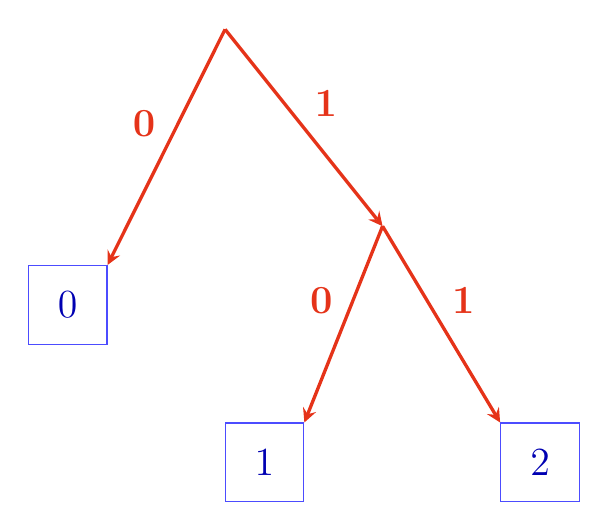
\begin{tikzpicture}[
  >=stealth,
  edge/.style={->, very thick, red!60!brown},
  lbl/.style={red!60!brown, font=\Large\bfseries},
  leaf/.style={draw=blue!70, text=blue!70!black, minimum size=1cm, font=\Large\bfseries}
]
  % nodes
  \coordinate (root) at (0,0);
  \coordinate (mid)  at (2,-2.5);
  \node[leaf] (n0) at (-2,-3.5) {$0$};
  \node[leaf] (n1) at (0.5,-5.5) {$1$};
  \node[leaf] (n2) at (4,-5.5) {$2$};

  % edges
  \draw[edge] (root) -- node[lbl, above left]  {0} (n0.north east);
  \draw[edge] (root) -- node[lbl, above right] {1} (mid);
  \draw[edge] (mid)  -- node[lbl, above left]  {0} (n1.north east);
  \draw[edge] (mid)  -- node[lbl, above right] {1} (n2.north west);
\end{tikzpicture}

See picture.

\subsection{Prefix code}

$X$ gets values in $\left\{1,\ldots,m\right\}$ with probabilities $\left(p_1,\ldots,p_m\right)$, we want to place the symbols $1,\ldots,m$ on the leaves of a binary tree (a tree with out-degree 0 or 2). Each symbol is coded by the bits on the path that leads to it. (Prefix code is where no codeword is a prefix of a different codeword).

See picture for example.

The average code length for a prefix code is given by
\[
L(T) = \sum_{i=1}^{m }p_i l_i,
\]
where $l_i$ is the length of path leading to symbol $i$ (number of bits used to code $i$).

We want the optimal code, the code that minimizes 
\[
\sum_{i=1 }^{m }p_i l_i 
\]
Using Huffman code we can get to average code length 
\[
H(p_1,\ldots, p_m)\leq \sum_{i=1 }^{m }p_i l_i < H(p_1,\ldots, p_m ) + 1
\]
and if $p_1,\ldots,p_,$ are powers of 2, the average code length is exactly $H(p_1,\ldots, p_m)$.

\subsection{The optimal code}

Suppose that a tree $T$ is optimal for symbols $\left\{1,\ldots, m\right\}$ with probabilities $\left(p_1,\ldots, p_m\right)$ (without loss of generality, we can assume $p_1\geq p_2\geq \cdots \geq p_m$).

Let $v$ do be the deepest non-leaf vertex in $T$. Since $T$ is optimal, w.l.o.g the symbols on the children of $v$ are $m-1,m$ (as otherwise we can change them to be $m-1,m$ without increasing $\sum_{i=1 }^{m }p_i l_i$)

See the picture.

Let $T'$ be the tree generated from $T$ by removing the children of $v$ and placing the new symbol $\ast=\left\{m-1,m\right\}$ on $v$. $T'$ is a tree (or code) for symbols $\left\{1,\ldots, m-2,\ast\right\}$, with probabilities $\left(p_1,\ldots, p_{m-2},p_{m-1}+p_m\right)$. We have 
\[
L(T) = L(T'1) + (p_{m-1}+p_m)\cdot 1
\]
Thus, $T$ is optimal for $\left\{1,\ldots, m\right\}$ with probabilities $\left(p_1\right)$ missed the rest

\subsection{Huffman's algorithm}

Input: $(p_1,\ldots, p_m)$ and sort them in descending order.

Find, by recursion, the best tree for probabilities $\left(p_1,\ldots, p_{m-2},p_{m-1}+p_m\right)$ see the picture for the rest

\subsubsection{Example}

See the picture 

\subsection{$L(T)$ when $p_1,\ldots,p_m$ are all powers of 2}

Lemma: If for every $i$, $p_i=2^{-d_i}$, then in Huffman's tree $T$: $l_i=d_i$.

See the photo for the example.

\subsubsection{First Proof}

Assume, w.l.o.g. $d_1\leq d_2\leq \cdots \leq d_m$. Then $d_m=d_{m-1}$, as otherwise,
\[
2^{d_m} = 2^{d_m}\cdot \sum_i p_i = \sum_i 2^{d_m}\cdot p_i = \sum_i 2^{d_m}\cdot 2^{-d_i}
\]
has even left-hand side and odd right-hand side.

Maybe more explicitly, we could write 
\[
\sum_i 2^{d_m}\cdot 2^{-d_i} = \sum^m_{i=1} 2^{d_m-d_i}= 1+ \sum^{m-1}_{i=1} 2^{d_m-d_i}
\]
where the right hand side would be odd if $d_{m-1}\neq d_m$.

\subsubsection{Second Proof}

Assume w.l.o.g. $d_1\leq d_2\leq \cdots \leq d_m$. Then $d_m=d_{m-1}$.

Thus $\left(p_1,\ldots,p_{m-2},p_{m+1}+p_m\right)$ are all powers of 2 and by induction the claim is true for $T'$ and hence also for $T$ when we replace the leaf that corresponds to $\left\{m-1,m\right\}$ by a vertex with two leaves.

Hence 
\[
\sum_{i=1 }^{m }p_i l_i = \sum_{i=1 }^{m }p_i d_i = \sum_{i=1 }^{m }p_i \log \frac{1 }{p_i }= H\left(p_1, \ldots, p_m \right) = H(X)
\]

\subsection{For every $T$, we have $H(X)\leq L(T)$}

Claim: For any binary tree $T$, with leaves $1,\ldots,m$
\[
\sum_{i=1 }^{m }2^{-l_i}=1
\]
where $l_i$ is the length of path to leaf $i$ and the sum is over all leaves.

See picture for example.

\subsubsection{Proof}

Consider a random walk from the root to the leaves that at each step goes from a non-leaf vertex $v$ to each of its two children with probability $1/2$ each, until reaching a leaf. Then the probability to reach leaf $i$ is $2^{-l_i}$ and since the random walk reaches exactly one leaf the total probability must be 1 (alternatively, a proof by induction).

\subsection{For every $T$, we have $H(X)\leq L(T)$}

Proof: For any binary tree $T$, with leaves $1,\ldots, m$ we now know $\sum_{i=1 }^{m }2^{-l_i}=1$, where $l_i$ is the length of path to leaf $i$. 

Let $q=\left(2^{-l_1}, \ldots, 2^{-l_m}\right)$. thus $q$ is a distribution over $\left\{1,\ldots, m\right\}$. We have 
\begin{align*}
    0\leq \operatorname{D}\left(p\vert q\right)&=\sum_i p_i\log\frac{p_i }{q_i}\\
    &= \sum_i p_i \log p_i + \sum_i p_i \log \left(\frac{1 }{q_i}\right)\\
    &= -H(X) +\sum_i p_i l_i
\end{align*}
Thus 
\[
H(X) \leq L(T)
\]

\subsection{$L(T) < H(X) +1 $}

We know the lower bound, but now we can find the upper bound (on an optimal code, Huffman's code).

First step of the proof, for every $i$, let $q_i=2^{-d_i}$ be the largest power of $2$ that is less than or equal to $p_i$. Thus, $\frac{p_i}{2}< q_i\leq p_i$. Note that $\sum_i q_i \leq 1$.

This means that $\left(q_1,\ldots,q_m\right)$ might not be a distribution, but we can fix this by extending.

Extend $q_1,\ldots,q_m$ to a distribution over $m'\geq m$ elements by adding $q_{m+1},\ldots,q_{m'}$ that are powers of 2. (We won't prove it, but it's not hard.)

Let $T$ be Huffman's tree for $q_1,\ldots,q_{m'}$. We use $T$ as a tree for $p_1,\ldots,p_m$ (by giving probability $0$ to symbols in $\left\{m+1,\ldots,m'\right\}$). Now we can write 
\begin{gather*}
    L(T) = \sum_{i=1 }^{m }p_i l_i = \sum_{i=1 }^{m }p_i d_i \\
    < \sum_{i=1 }^{m }p_i \log \frac{1 }{p_i/2 }= \sum_{i=1 }^{m }p_i \left(\log \frac{1 }{p_i }+ 1 \right)= H(X) + 1
\end{gather*}
Since Huffman's tree is optimal, this must be true also for Huffman's.

\subsection{Back to Huffman's code (a prefix code)}

$X$: a discrete random variabel (finite number of states)

Theorem: Alice can encode $X$ using less than $H(X)+1$ bits \textit{in expectation}. From this encoding, Bob can retrieve $X$ with probability 1.

\textbf{Corollary}: By Markov's inequality, Alice can encode $X$ using $\mathcal{O}\left(H(X)\right)$ bits, in the worst case. From this encoding, Bob can retrieve $X$ with probability $1-\epsilon$.

\section{Review: Approximating Multinomial Coefficients}

Let $\left(p_1,\ldots,p_m\right)$ be a distribution and thus $\sum_{i=1 }^{m }p_i=1$. Let $n\in \mathbb{N }$ and let $\left(n_1,\ldots,n_m\right)$ be such that $n_i=np_i$ and thus $\sum_{i=1 }^{m }n_i=n$. Consider the multinomial coefficient
\[
\frac{n !}{n_1 !\cdot n_2 ! \cdot \ldots \cdot n_m!} = \frac{n!}{(np_1)!\cdot (np_2)!\cdot\ldots \cdot (np_m)!}
\]
As $n\to\infty$, we can write 
\[
\frac{1}{n}\cdot \log\left(\cdots\right)
\]
see the picture.

\section{Data Compression}

\subsection{Example}

Let $X_1,\ldots,X_n$ be independent random variables, such that, each $X_i$ is 0 with probability $p$ and 1 with probability $1-p$.

With high probability, about $pn$ of them are $0$. Assume that exactly $k=pn$ of them are $0$ and $\left(1-p\right)n$ are 1. Then, the number of possibilities for $X_1,\ldots, X_n$ is $\binom{n }{k }\approx 2^{n\cdot H\left(p,1-p\right)}$.

Thus, around $n\cdot H(p,1-p)$ bits are needed to tell in which possibility we are, and hence to describe the values of $X_1,\ldots,X_n$
\[
n\cdot H(p,1-p)= n\cdot H(X_i)=H(X_1,\ldots,H_n)
\]

\subsubsection{A Protocol for Describing $X_1,\ldots,X_n$}
If $X_1,\ldots,X_n$ are i.i.d and $X_i$ has the distribution $\left(p,1-p\right)$:
\begin{enumerate}
    \item Send the number of zeros: $k=n-\sum X_i\approx pn$ (with high probability ): $\log n$ bits (negligible)
    \item Send the exact values of $X_1,\ldots,X_n$, among all possibilities with $k$ zeros: $\approx n\cdot H(p,1-p)$ bits
\end{enumerate}

\subsection{More generally}

If $X_1,\ldots,X_n$ are i.i.d and $X_i$ has the distribution $\left(p_1,\ldots, p_m\right)$, where $n >> m \, \left(n\to \infty\right)$, we can describe $X_1,\ldots, X_n$ but sending about $n\cdot H(p_1,\ldots,p_m)$ bits:
\begin{enumerate}
    \item Send the empirical distribution $\left(n_1,\ldots, n_m\right)$, where $n_i\approx p_i n$ is the number of $X_j$-s that have the value $i$: $m\log n$ bits (negligible)
    \item Send the exact values of $X_1,\ldots, X_n$ among all possibilities with that empirical distribution: $\approx n\cdot H(p_1,\ldots,p_m)$ bits
\end{enumerate}

\subsection{Shannon's Source Coding Theorem}

If $X_1,\ldots,X_n$ are independent and identically distributed, Alice can encode $X_1,\ldots,X_n$ using $H(X_i)\cdot n + \mathcal{o }(n)$ bits (in the worst case). From this encoding, Bob can retrieve $X_1,\ldots, X_n$ with probability $1-\mathcal{o }(1)$.

(Both Alice and Bob know the distribution of $X_1,\ldots, X_n$)

We will give a more formal general proof that proves even more than that (using the Asymptotic Equipartition Theorem).

Similar theorems, that roughly $H(X_1,\ldots, X_n)$ bits are needed to describe all variables $X_1,\ldots, X_n$, are also true in more general settings (such as Markov chains and other stochastic processes).

\section{Asymptotic Equipartition Theorem}

\subsection{Law of Large Numbers}

If $Z_1,\ldots,Z_n$ are i.i.d, then 
\[
\frac{Z_1 + \cdots + Z_n}{n}\to \mathbb{E}(Z_i)
\]
(convergence in distribution equals convergence of the cumulative distribution function). That is, for every $\epsilon > 0$,
\[
P_{Z_1,\ldots,Z_n}\left[ | \frac{Z_1 + \cdots + Z_n}{n} - \mathbb{E}(Z_i) |>\epsilon \right] \to 0
\]

\subsection{Asymptotic Equipartition Theorem: Informal}

Let $X_1,\ldots,X_n$ be i.i.d. Consider the random variable $-\log P\left(X_1,\ldots, X_n\right)$. Note that $\mathbb{E}\left(-\log P\left(X_1,\ldots, X_n\right) \right)=H(X_1,\ldots,X_n)$. We will show that almost always $-\log P\left(X_1,\ldots, X_n\right)$ is very close to its expectation.

\subsection{Asymptotic Equipartition Theorem: Formal}

If $X_1,\ldots, X_n$ are i.i.d, then 
\[
\frac{-\log P(X_1,\ldots, X_n)}{n}\to H(X_i)
\]
(convergence in distribution equals convergence of the cumulative distribution function). That is, for every $\epsilon > 0$,
\[
P_{Z_1,\ldots,Z_n}\left[ | \frac{-\log P(X_1,\ldots, X_n)}{n} - H(X_i) |>\epsilon \right] \to 0
\]

\subsubsection{Proof}

Since $X_1,\ldots,X_n$ are independent,
\[
P(X_1,\ldots,X_n)=P(X_1)\cdot\ldots\cdot P(X_n)
\]
Hence by the law of large numbers 
\[
\frac{-\log P(X_1,\ldots, X_n)}{n}  = \frac{-\sum_i \log P(X_i)}{n}\to \mathbb{E}\left(-\log P(X_i)\right)=H(X_i)
\]

\subsection{Additional Form: I}

If $X_1,\ldots, X_n$ are i.i.d, then 
\[
P_{Z_1,\ldots,Z_n}\left[ | \frac{-\log P(X_1,\ldots, X_n)}{n} - H(X_i) |>\epsilon \right] \to 0
\]
which implies 
\[
P\left[ H(X_i)-\epsilon \leq \frac{-\log P(X_1,\ldots, X_n)}{n} \leq H(X_i) + \epsilon \right] \to 1
\]
\[
P\left[ 2^{H(X_i)-\epsilon} \leq \frac{-\log P(X_1,\ldots, X_n)}{n} \leq H(X_i) + \epsilon \right] \to 1
\]
See the picture.

Thus, $P(X_1,\ldots,X_n)$ is with high probability close to $2^{-H\left(X_1,\ldots,X_n\right)}$

\subsection{Additional Form: II}

Let $X_1,\ldots,X_n$ be i.i.d. Let $X=\left(X_1,\ldots,X_n\right)$. For every $n$ and $\epsilon>0$, denote by $A_{n,\epsilon}$ the set of ``typical sequences'':
\[
A_{n,\epsilon}=\left\{a=\left(a_1,\ldots, a_n\right)\Big| 2^{-n\cdot \left(H(X_i) + \epsilon\right)}\leq P(X=a) \leq 2^{-n\cdot \left(H(X_i)-\epsilon\right)}\right\}
\]
See the picture.

\section{Data Compression}

We think of $A_{n,\epsilon}$ as the set of states that $\left(X_1,\ldots,X_n\right)$ can take (as the rest is negligible and will result in negligible error). We have 
\[
| A_{n,\epsilon} | \approx 2^{H(X_1,\ldots,X_n)}
\]
Alice can describe $\left(X_1,\ldots, X_n\right)$ by sending about $H(X_1,\ldots, X_n)$ bits. From this description, Bob can recover $\left(X_1,\ldots, X_n\right)$ exactly, with high probability.

This is called Shannon's Source Coding Theorem. There are similar theorems for non i.i.d conditions.

\subsection{Lower Bound}

Is Shannon's source coding theorem tight?

Could Alice send significantly less than $H\left(X_1,\ldots,X_n\right)$ bits from which Bob ... lost the rest

\subsubsection{Proof}

For simplicity, assume that $X_1,\ldots, X_n$ are bits. Assume that Alice encodes $X=\left(X_1,\ldots, X_n \right)$ by applying a function $f$ and obtains $Y=f(x)$. Assume that $Y$ is of length $m$ bits. Assume that from $Y$, Bob recovers $X$ with high probability by applying a function $g$, obtaining $g(Y)$
\[
X\to f(X)\to g(f(X))
\]
Assume that $P(X=g(Y))\geq 1-\epsilon$.

By Question 9 in Problem Set 1\footnote{There was a hint of constructing an indicator variable.},
\[
H(X|Y) \leq H(\epsilon, 1-\epsilon) + \epsilon n < \epsilon n + 1
\]
We hence have,
\begin{gather*}
    I(X;Y) = H(Y) - H(Y|X)\leq H(Y) \leq m \\
    I(X;Y) = H(X) - H(X|Y) > H(X) -\epsilon n - 1
\end{gather*}
Thus,
\[
m > H(X) -\epsilon n - 1
\]
This is an example of the power of the equalities and inequalities of information theory


\end{document}